
\chapter*{Teil 0 -- Wie dieses Buch funktioniert}
\addcontentsline{toc}{chapter}{Teil 0 -- Wie dieses Buch funktioniert}
\markboth{Wie dieses Buch funktioniert}{}

Liebe Julia,

das hier ist kein Lehrbuch, das dich langweilen will. Es ist eine Einladung:
an Straßenschilder, Taxifahrer, Kaffeehausbesitzer und mindestens eine sehr
selbstbewusste Straßenkatze namens Bisso. Los geht's -- ganz von vorne, ganz
in Ruhe.

\section*{Was du hier lernst: ganz normales, gesprochenes Arabisch}

Arabisch hat zwei Ebenen: eine Schriftsprache für Nachrichten und Bücher
(Fus'Ha), und die Sprache, die 90 Millionen Menschen in Kairo tatsächlich
\emph{sprechen} (Masri, Ägyptisch-Arabisch). \textbf{Dieses Buch
konzentriert sich fast komplett auf Masri} -- das normale, entspannte
Alltagsarabisch, das du beim Taxifahren, im Café und beim Feilschen
brauchst. Nur an wenigen Stellen zeigen wir dir kurz den Fus'Ha-Unterschied,
falls du ihn mal auf einem Schild siehst.

\begin{tippbox}
Du musst dir jetzt noch \emph{gar keine} Sorgen um ,,zwei Sprachen`` machen.
Für den Anfang gilt: lern die Wörter in diesem Buch so, wie sie dastehen --
das ist genau das Arabisch, das echte Menschen in Ägypten mit dir sprechen
werden.
\end{tippbox}

\section*{Die Julia-Umschrift}

Arabisch hat Laute, die es im Deutschen nicht gibt -- aber du hast einen
Heimvorteil: Deutsch besitzt bereits zwei Laute, an denen Englischsprachige verzweifeln.

\begin{center}
\renewcommand{\arraystretch}{1.4}
\begin{tabular}{cll}
\textbf{Zeichen} & \textbf{Beispiel} & \textbf{Eselsbrücke} \\
\hline
ch & \textit{chal\'as} & wie \textbf{ch} in ,,Ba\textbf{ch}`` \\
sch & \textit{sch\'ukran} & wie \textbf{sch} in ,,\textbf{Sch}ule`` \\
g & \textit{gam\'il} & wie \textbf{g} in ,,\textbf{g}eben`` -- ägyptisch, nie ,,dsch``! \\
' & \textit{'ahwa} & ein kleiner Stopp, wie in ,,Spiegel-\textbf{ei}`` \\
3 & \textit{3\'ayez} & ein Laut tief aus dem Hals \\
H & \textit{aHmed} & ein heißes, geflüstertes H \\
\end{tabular}
\end{center}

Betonte Silben tragen einen Akzent (\textit{chal\'as}). Mehr brauchst du
nicht, um loszulegen.

\section*{Die Symbole in diesem Buch}

\begin{center}
\renewcommand{\arraystretch}{1.5}
\begin{tabular}{cl}
\textcolor{yallateal}{\faVolumeUp} & Tippen -> Google Translate öffnet sich -> Lautsprecher-Symbol tippen -> hören \\
\faHeart & Mohameds eigene Stimme (folgt in einer späteren Version) \\
\faLightbulb & Insider-Tipp für Ägypten \\
\faSmileWink & Lach-Pause \\
\faTaxi & Am Mahmoud, der Taxifahrer, hat etwas zu sagen \\
\faPaw & Bisso, die Straßenkatze, hat eine Meinung \\
\faFlagCheckered & Checkpoint -- kurz prüfen, ob's sitzt \\
\end{tabular}
\end{center}

\begin{tippbox}
Das \textcolor{yallateal}{\faVolumeUp}-Symbol öffnet Google Translate mit
dem Wort schon eingetragen -- Standardaussprache, sehr nützlich, aber nicht
immer der ägyptische Klang. Für die Wörter mit \faHeart\ gibt es später
eine Aufnahme von genau der Person, mit der du sie eigentlich sprechen
willst. Zum Antippen brauchst du eine Internetverbindung und einen
PDF-Betrachter, der Links öffnet (z.B. am Handy oder im Browser).
\end{tippbox}

\section*{Die Besetzung}

\begin{ammahmoudbox}
\textbf{Am Mahmoud} fährt seit 30 Jahren Taxi in Kairo, kennt jeden Umweg
und jeden Trick, und ist der Meinung, dass jeder Preis Verhandlungssache
ist. Sein Porträt folgt in einer späteren Version.
\end{ammahmoudbox}

\begin{bissobox}
\textbf{Bisso} ist eine Straßenkatze mit einer eingekerbten Ohrspitze und
starken Meinungen zu Essensresten.
\end{bissobox}

\begin{center}
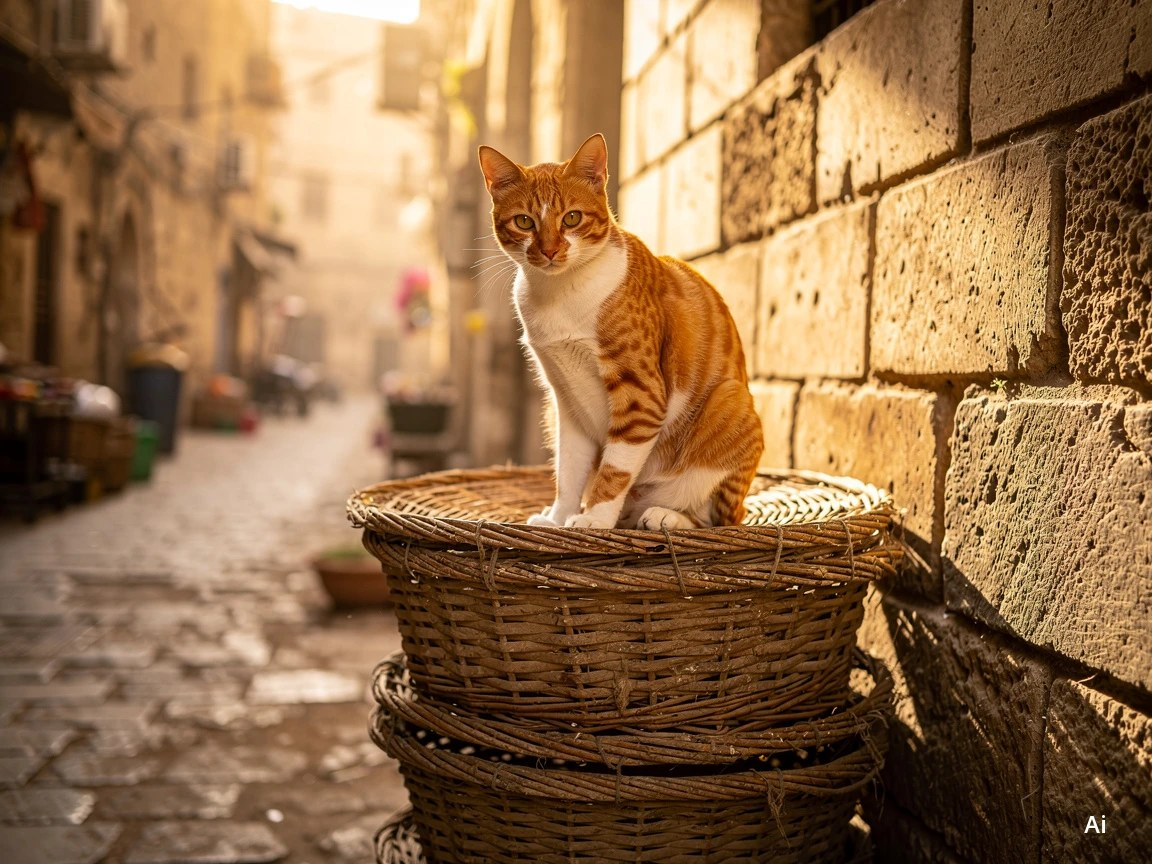
\includegraphics[width=0.5\textwidth]{images/bisso.jpg}\\
{\small\itshape Bisso, wie sie wirklich aussieht (ja, wirklich).}
\end{center}

Bereit? \textarabic{يلا بينا!} (\textit{yalla beena} -- ,,los geht's, wir beide!``)
